\section{Conectarea la un server}
Pentru a evidentia capacitatile de comunicare, vom realiza o conexiune tcp la un server si vom trimite si primi date de la acesta.
\paragraph{Permisiuni} Pentru a realiza conexiuni la internet, trebuie sa adaugam permisiunea in fisierul AndroidManifest.xml:
\begin{lstlisting}[language=XML]
...
<uses-permission android:name="android.permission.INTERNET" />
...
\end{lstlisting}
In fragmentul \texttt{fragment\_communication.xml} am adaugat elementele de interfata necesare pentru a realiza conexiunea la server.
In clasa viewmodel corespunzatoare avem nevoie de un string in care sa stocam raspunsul primit de la server.
Va trebuii sa observam schimbarile din acest string si sa le afisam in interfata grafica.
\begin{lstlisting}[language=Kotlin]
 override fun onCreateView(
        inflater: LayoutInflater,
        container: ViewGroup?,
        savedInstanceState: Bundle?
    ): View {
        ...
        communicationViewModel.response.observe (viewLifecycleOwner) {
            binding.responseText.text = it
        }
        ...
    }
\end{lstlisting}
\paragraph{Conectarea la server} In metoda \texttt{onCreateView} vom adauga un listener pentru butonul de send.
Pentru a realiza conexiunea la server, vom folosi clasa \texttt{Socket}. Deoarece
aceasta clasa nu poate fi folosita in thread-ul principal, vom folosi un thread separat pentru a realiza conexiunea.
\begin{lstlisting}[language=Kotlin]

 binding.button2.setOnClickListener {
            val network_thread = Thread {
                Log.d("WIFI", "Clicked send tcp")
                val address: String = binding.addrText.text.toString()
                val port: Int = binding.portText.text.toString().toInt()
                val connstr = "$address:$port";

                Log.d("WIFI", "Clicked send tcp, connecting to $connstr")
                val client = Socket(address, port)
                Log.d("WIFI", "Sending the message")
                val data = binding.messageText.text.toString() + '\n'
                client.getOutputStream().write(data.toByteArray())
                Log.d("WIFI", "MessageSent, waiting for response")
                val scanner = Scanner(client.getInputStream())
                val resp = scanner.nextLine()
                Log.d("WIFI", "Got response!$resp")
                communicationViewModel.onResponse(resp)
            }
            network_thread.start()
        }
\end{lstlisting}

Valorile pentru adresa si portul serverului sunt citite din interfata grafica, valorile implicite au fost setate pentru conectarea
la serverul \texttt{tcpbin}, care este un server ce returneaza datele primite, acestea trebuie sa fie terminate cu un caracter de newline.

\begin{figure}[H]
    \begin{subfigure}{0.5\textwidth}
        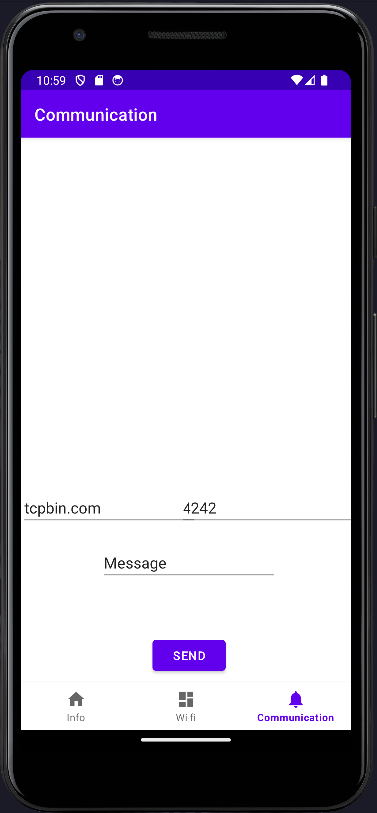
\includegraphics[width=\textwidth]{figs/comm_before.png}
    \end{subfigure}
    \hfill
    \begin{subfigure}{0.5\textwidth}
        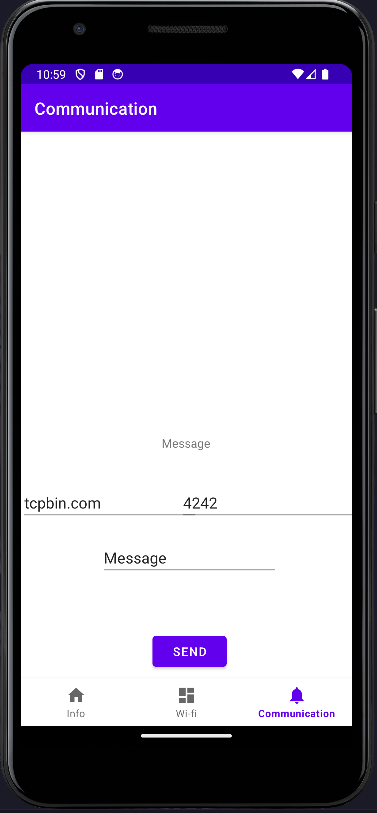
\includegraphics[width=\textwidth]{figs/comm_after.png}
    \end{subfigure}
\end{figure}